\documentclass{article}

\usepackage{amsmath}
\usepackage{amsfonts}
\usepackage{amssymb}
\usepackage{amscd}
\usepackage{amsthm}
\usepackage{graphics}
\usepackage{graphicx}
\usepackage{tikz}
\usepackage{biblatex}

\addbibresource{auxetic.bib}
\graphicspath{ {./} }

\title{Patient-Specific Artificial Intestine: Biomechanics of Auxetic Structures}
\author{Daniel Wei, Mingruifu Lin}
\date{February 2025}

\begin{document}

\maketitle

\begin{abstract}
  Colorectal cancer (CRC) is the third most commonly diagnosed cancer globally, with over 1.9 million new cases and approximately 930,000 deaths estimated in 2020. PubMed Despite advancements in tissue engineering, current research predominantly focuses on replicating the intestinal absorption layer, with limited progress in recreating the muscular layer essential for bowel motility. In effect, the organicity of biological macrostructures often cannot be broken down effectively into manufacturable units. Current solutions like colostomy bags are impractical and fail to fully replicate natural intestinal function, highlighting the need for more functional alternatives. PMC This research aims to develop a bio-inspired, patient-specific artificial intestine that can be folded from a flat auxetic lattice generated upon the input of a desired 3D shape (such as a colon), which approximates smooth peristaltic movements through expansion and contraction from each auxetic unit. The algorithm can be generalized for other applications beyond prostheses. A combination of computational testing and visualization, and 3D printed prototypes are used to verify the method's effectiveness. The result of this research is an algorithm that processes data from the scanned model of a colon to generate a 3D printable flat mesh that morphs under the propagation of tension or compression along multiple control units located on its boundary. By the 2D nature of the printed surface which folds into 3D, the research impacts material engineering by preventing problems related to supports in 3D printing involving more vertical structures, allowing for more complex shapes to occur. Also, it gives options for the development of new types of prostheses that better reproduce organic movement. When combined with advanced absorption layer technologies, this approach provides an efficient solution to the production of artificial intestines and other similar organs.

  \textbf{Keywords}: Artificial intestine, patient-specific design, biomechanics, auxetic materials, material engineering, 3D printing, 3D models, parametric surfaces
\end{abstract}

\pagebreak

\tableofcontents

\pagebreak

\section{Introduction}
The development of artificial intestines presents a major challenge in tissue
engineering. Current approaches focus primarily on absorption rather than
replicating the biomechanical movements necessary for digestion. This project
seeks to address that gap through the use of auxetic structures to mimic natural
peristaltic motion. The main objective is to generate a 3D printable auxetic
mesh that folds into a functional artificial intestine.

\section{Materials and Methods}
This research utilizes computational modeling and 3D printing to develop and
test auxetic lattice structures. The process includes:
\begin{enumerate}
  \item Importing scanned colon models into a computational pipeline.
  \item Converting the 3D model into a flat auxetic lattice through a custom algorithm.
  \item Simulating peristaltic motion and validating material properties.
  \item 3D printing and evaluating prototypes for structural integrity and movement accuracy.
\end{enumerate}

\section{Outline of Algorithm}
The algorithm takes in a triangulated mesh with a simple-enough, well-behaved topology, and outputs the information necessary to generate a 3D printable auxetic mesh that folds into the desired original mesh. We were inspired by Tachi's presentation. \cite{tachi}

\subsection{Boundary}
Boundary identification for a connected topological disk can be done with the usual method that checks for edges having only a single adjacent face. Then, the boundary vertices are ordered into a loop, which is mapped to a square or rectangle on a plane. Other shapes, such as cylinders or sphere, must be incised into a connected topological disk. For example, a topological cylinder can be incised along its height, while a topological sphere can be incised along a half-circumference.

\subsection{Parametrization}
We use barycentric mapping, and the idea is to treat edges as springs, and calculate their equilibrium length on a flat plane. If we take $0$ as the equilibrium length of a spring, then the spring energy between two vertices with spring constant $D$ is given as follow:
$$E_{ij} = \frac{1}{2} D \lVert \Delta \vec{x} \rVert ^2 = \frac{1}{2} D \lVert \vec{x}_i - \vec{x}_j \rVert ^2$$
The total spring energy is thus:
$$E = \frac{1}{2} \sum_{i} \sum_{j \in N_i} \frac{1}{2} D_{ij} \lVert \vec{u}_i - \vec{u}_j \rVert ^2$$
where each $\vec{u}_i$ lies on the 2D plane, and $N_i$ are the neighboring vertices of $i$. The fraction $\frac{1}{2}$ at the beginning is added because each edge is counted twice in this formula. Notice that $E$ is a scalar field depending on the position of each vertex. The idea is to minimize the spring energy, so we want the derivative to be zero for each parameter:
$$\frac{\partial E}{\partial \vec{u}_i} = \vec{0}$$
which is a fancy notation for gradient with respect to $\vec{u}_i$. Doing the computation, we get:
$$\frac{\partial E}{\partial \vec{u}_i} = \sum_{j \in N_i} D_{ij} (\vec{u}_i - \vec{u}_j) = \vec{0}$$
Notice that the fraction $\frac{1}{2}$ is not required anymore, because we are not counting edges twice. Anyways, we see that:
$$\sum_{j \in N_i} D_{ij} \vec{u}_i = \sum_{j \in N_i} D_{ij} \vec{u}_j$$
Hence,
$$\vec{u}_i = \frac{\sum_{j \in N_i} D_{ij} \vec{u}_j}{\sum_{j \in N_i} D_{ij}}$$
Rewritten:
$$\vec{u}_i = \sum_{j \in N_i} \lambda_{ij} \vec{u}_j$$
where $\lambda_{ij} = \frac{D_{ij}}{\sum_{k \in N_i} D_{ik}}$, we then isolate the constant terms, which are the things that involve the boundary vertices:
$$\vec{u}_i - \sum_{j \in N_i, j \leq n} \lambda_{ij} \vec{u}_j = \sum_{j \in N_i, j > n} \lambda_{ij} \vec{u}_j$$
where the boundary vertices are counted with indices after $n$. We can go component-wise. Let $u_k$ and $v_k$ be the coordinates of the 2D vertex $\vec{u}_k$, then we can write:
$$u_i - \sum_{j \in N_i, j \leq n} \lambda_{ij} u_j = \sum_{j \in N_i, j > n} \lambda_{ij} u_j$$
$$v_i - \sum_{j \in N_i, j \leq n} \lambda_{ij} v_j = \sum_{j \in N_i, j > n} \lambda_{ij} v_j$$
Let us consider only the first coordinate of the vertices. I can rewrite like this:
$$\begin{pmatrix}
  1 & -\lambda_{12} \text{ or 0} & -\lambda_{13} \text{ or 0} & \cdots & \lambda_{1n} \text{ or 0} \\
  -\lambda_{21} \text{ or 0} & 1 & -\lambda_{23} \text{ or 0} & \cdots & \lambda_{2n} \text{ or 0} \\
  -\lambda_{31} \text{ or 0} & -\lambda_{32} \text{ or 0} & 1 & \cdots & \lambda_{3n} \text{ or 0} \\
  \vdots & \vdots & \vdots & \ddots & \vdots \\
  -\lambda_{n1} \text{ or 0} & -\lambda_{n2} \text{ or 0} & -\lambda_{n3} \text{ or 0} & \cdots & 1\\
\end{pmatrix}
\begin{pmatrix}
  u_1 \\
  u_2 \\
  u_3 \\
  \vdots \\
  u_n
\end{pmatrix}
= \begin{pmatrix}
  a_1 \\
  a_2 \\
  a_3 \\
  \vdots \\
  a_n
\end{pmatrix}$$
where each $a_k = \sum_{j \in N_k, j > n} \lambda_{kj} v_j$ is just the RHS of our previous equation. As you see, some components of the matrix are either $\lambda_{ij}$ or $0$, depending on whether $j \in N_i$. We can do the same procedure for the vertical coordinates $v_i$. Notice that $a_i$ are zero if $\vec{u}_i$ is not a neighbor of a boundary vertex.

In any case, we have found a way to parametrize any mesh. \cite{meshparam} Solving the linear systems can be done by a library.

\subsection{Choice of metric}
For our algorithm, we chose $D_{ij} = \frac{1}{\lVert \vec{u}_i - \vec{u}_j \rVert}$. This is reminescent of the Newton per meter.

\subsection{Auxetics}
To determine the maximum rotation of an auxetic unit centered at $\vec{u}_i$, we will cap it to the smallest internal angle of its adjacent triangles:
$$\phi_i = \min\{\theta_{j, i, j + 1} \; \mid \; j \in N_i\}$$
where $\theta_{abc}$ means the angle formed by the points $\vec{u}_a, \vec{u}_b, \vec{u}_c$. We will always engineer the auxetic unit to make the biggest rotation.

To determine the maximum radius of the same auxetic unit, we take the minimum of half the distance to each neighbor:

$$R_i = \min\{\frac{\lVert \vec{u}_i - \vec{u}_j \rVert}{2} \; \mid \; j \in N_i\}$$

Radius capping shouldn't happen frequently, since our previously-discussed parametrization aims to be the most optimal. Also, in reality, we will actually cap it smaller to $\frac{1}{3}$, because we need to leave space for the rods between auxetic units.

To determine the knob's placement radius for each of the rods that will connect to the unit, we use the difference in length between the edge of the parametrized mesh and the original mesh.

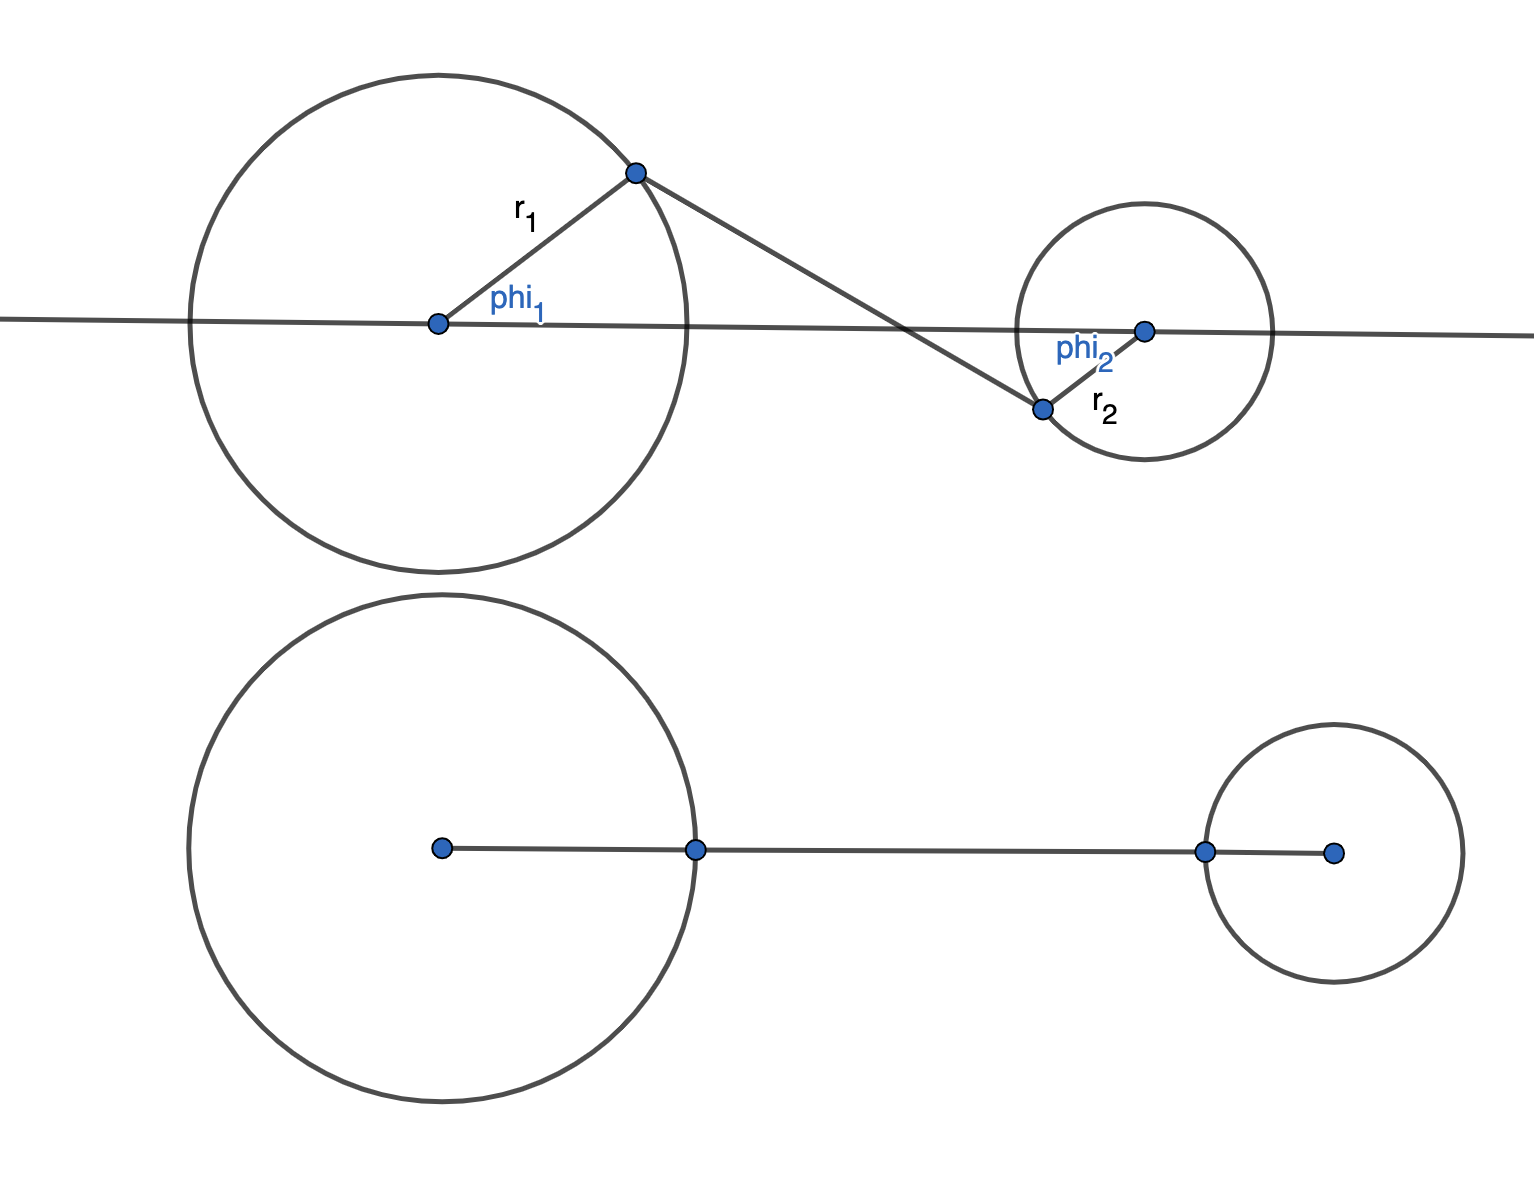
\includegraphics[scale=0.18]{geo-calc.png}

Let $r$ be the radius at which we want to place the knob, then we want:
$$r + \sqrt{(\frac{E}{2} - r \cos \phi_1)^2 + (r \sin \phi_1)^2} - \frac{E}{2} = \Delta_{ij}$$
where $\Delta_{ij}$ is the difference in length between the parametrized edge and the original edge, and $E$ is the length of the parametrized edge (length connecting the centers of the circles in the upper picture, the lower is the extended version). Thus, solving for $r$, we get:
$$r (E \cos \phi_1 - 2(\Delta_{ij} + \frac{E}{2})) = \frac{E^2}{4} - (D + \frac{E}{2})^2$$
If $r$ protrudes out of the unit, then we cap it to $R_i$.

Now, we have all the information needed to produce a printable mesh.

\section{Morphing}
$$\sum_{j \in N_1} r^j \vec{d}^{j} = \vec{F}^{ext1}$$
$$\sum_{j \in N_2} r^j \vec{d}^{j} = \vec{F}^{ext2}$$
$$\vdots$$
and so on, where $r^j$ is the magnitude of force we are solving, and $\vec{d}^j$ is the direction vector between two units.

Separating into $x$, $y$, $z$ components, we have the following linear system:
$$\begin{pmatrix}
  d^{1}_1 \text{ or 0} & d^{2}_1 \text{ or 0} & d^{3}_1 \text{ or 0} & \cdots & d^{n}_1 \text{ or 0} \\
  d^{1}_2 \text{ or 0} & d^{2}_2 \text{ or 0} & d^{3}_2 \text{ or 0} & \cdots & d^{n}_2 \text{ or 0} \\
  d^{1}_3 \text{ or 0} & d^{2}_3 \text{ or 0} & d^{3}_3 \text{ or 0} & \cdots & d^{n}_3 \text{ or 0} \\
  \vdots & \vdots & \vdots & \ddots & \vdots \\
  d^{1}_3 \text{ or 0} & d^{2}_3 \text{ or 0} & d^3_3 \text{ or 0} & \cdots & d^n_3 \text{ or 0} \\
\end{pmatrix}
\begin{pmatrix}
  r^1 \\
  r^2 \\
  r^3 \\
  \vdots \\
  r^n
\end{pmatrix}
= \begin{pmatrix}
  F^{ext1}_1 \\
  F^{ext1}_2 \\
  F^{ext1}_3 \\
  F^{ext2}_1 \\
  F^{ext2}_2 \\
  F^{ext2}_3 \\
  \vdots \\
  F^{extm}_1 \\
  F^{extm}_2 \\
  F^{extm}_3 \\
\end{pmatrix}$$

\section{Results and Discussion}
Through computational modeling, the project successfully developed an auxetic
lattice capable of transforming into a functional artificial intestine. Results
showed that:
\begin{enumerate}
  \item The algorithm generalizes to different intestine sizes and patient-specific needs.
  \item Prototypes demonstrated the feasibility of 3D printing complex auxetic structures.
\end{enumerate}

Challenges included ensuring the printed structure’s durability and fine-tuning
material properties to match biological tissues. Future work involves refining
the computational model to optimize mechanical performance and exploring
biocompatible materials.

\section{Software Details}

\subsection{OBJ Graph Conversion}
Our software only uses OBJ, since they are simple file formats. Graph conversion is simple, so we will skip its description here.

\subsection{Boundary Settings}
Difference starting vertices for the ordering of the boundary produces vastly different flat parametrizations. The software allows you to choose the starting vertex, as well as the width and height of the parametrized boundary square/rectangle.

\subsection{3D Models}
Here are pictures of the mechanical joints used in the printable mesh.

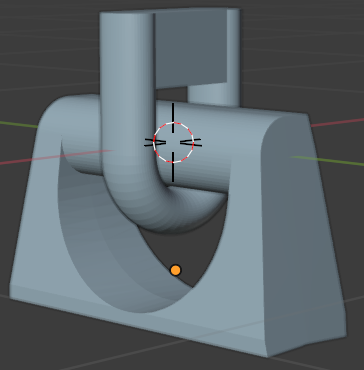
\includegraphics[scale=0.3]{knob.png}
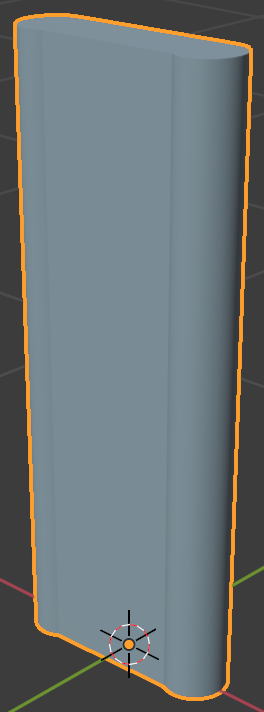
\includegraphics[scale=0.3]{rod.png}

\section{Conclusion}
The study demonstrates a novel approach to designing artificial intestines by
leveraging auxetic structures. The proposed solution offers improved biomechanical functionality and the potential for customization based on patient
needs. Future work includes expanding the methodology to other prosthetic
applications.

\subsection{Examples}

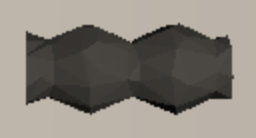
\includegraphics[scale=1.2]{example3.png}

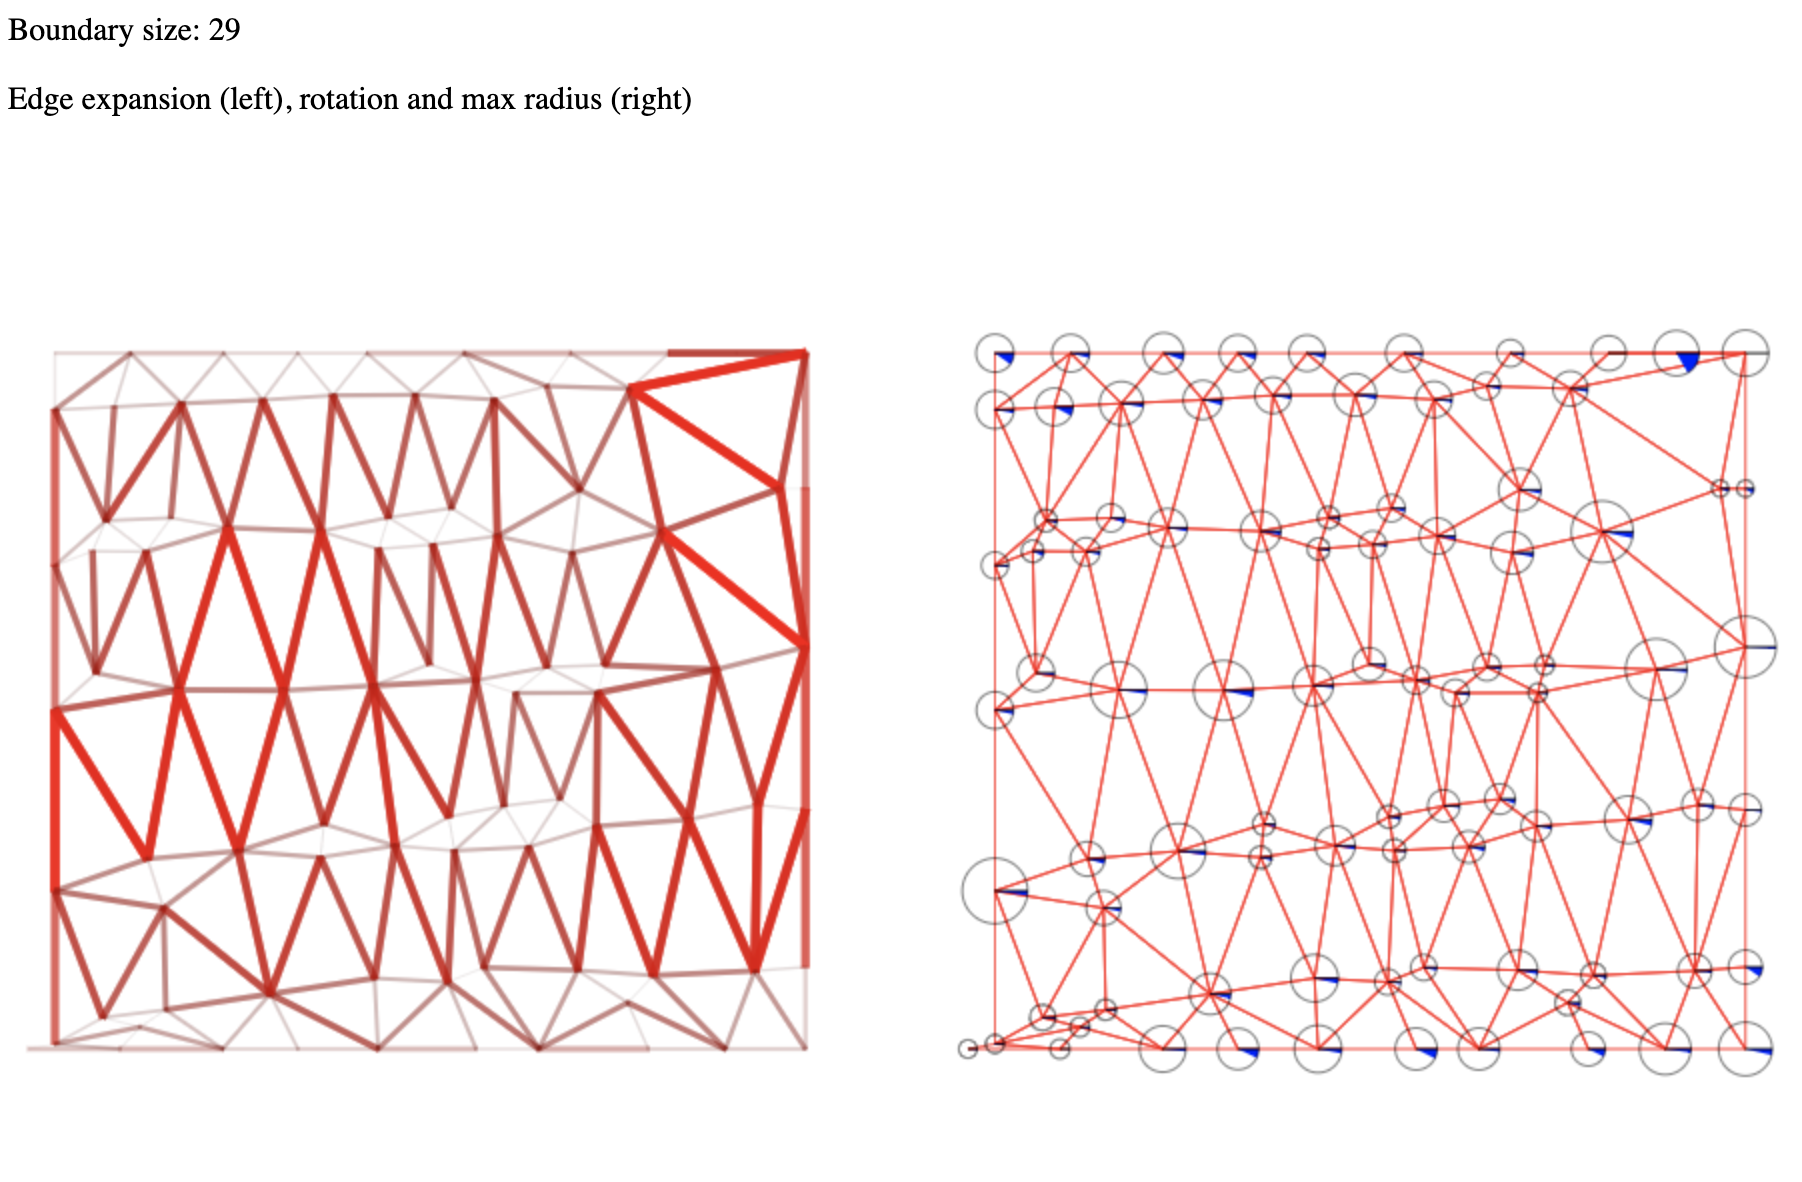
\includegraphics[scale=0.18]{example2.png}

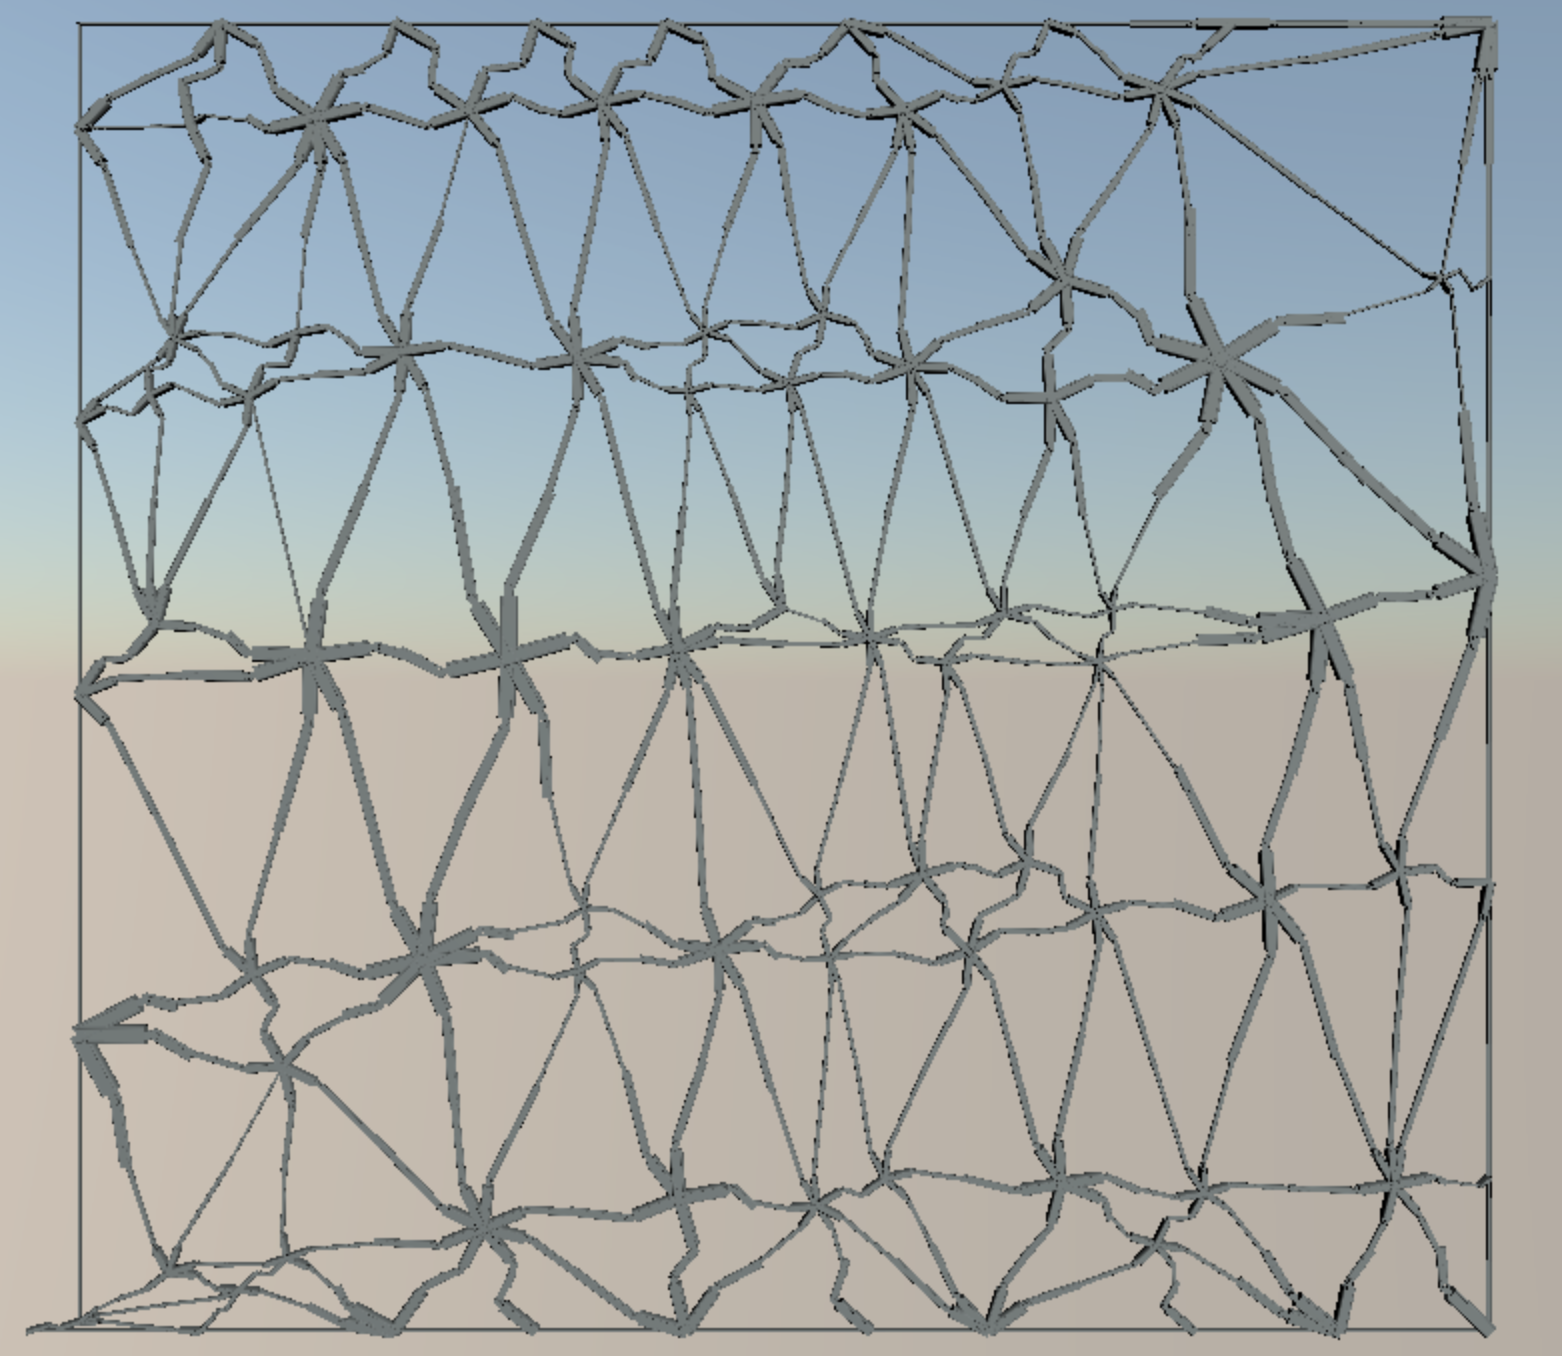
\includegraphics[scale=0.18]{example0.png}

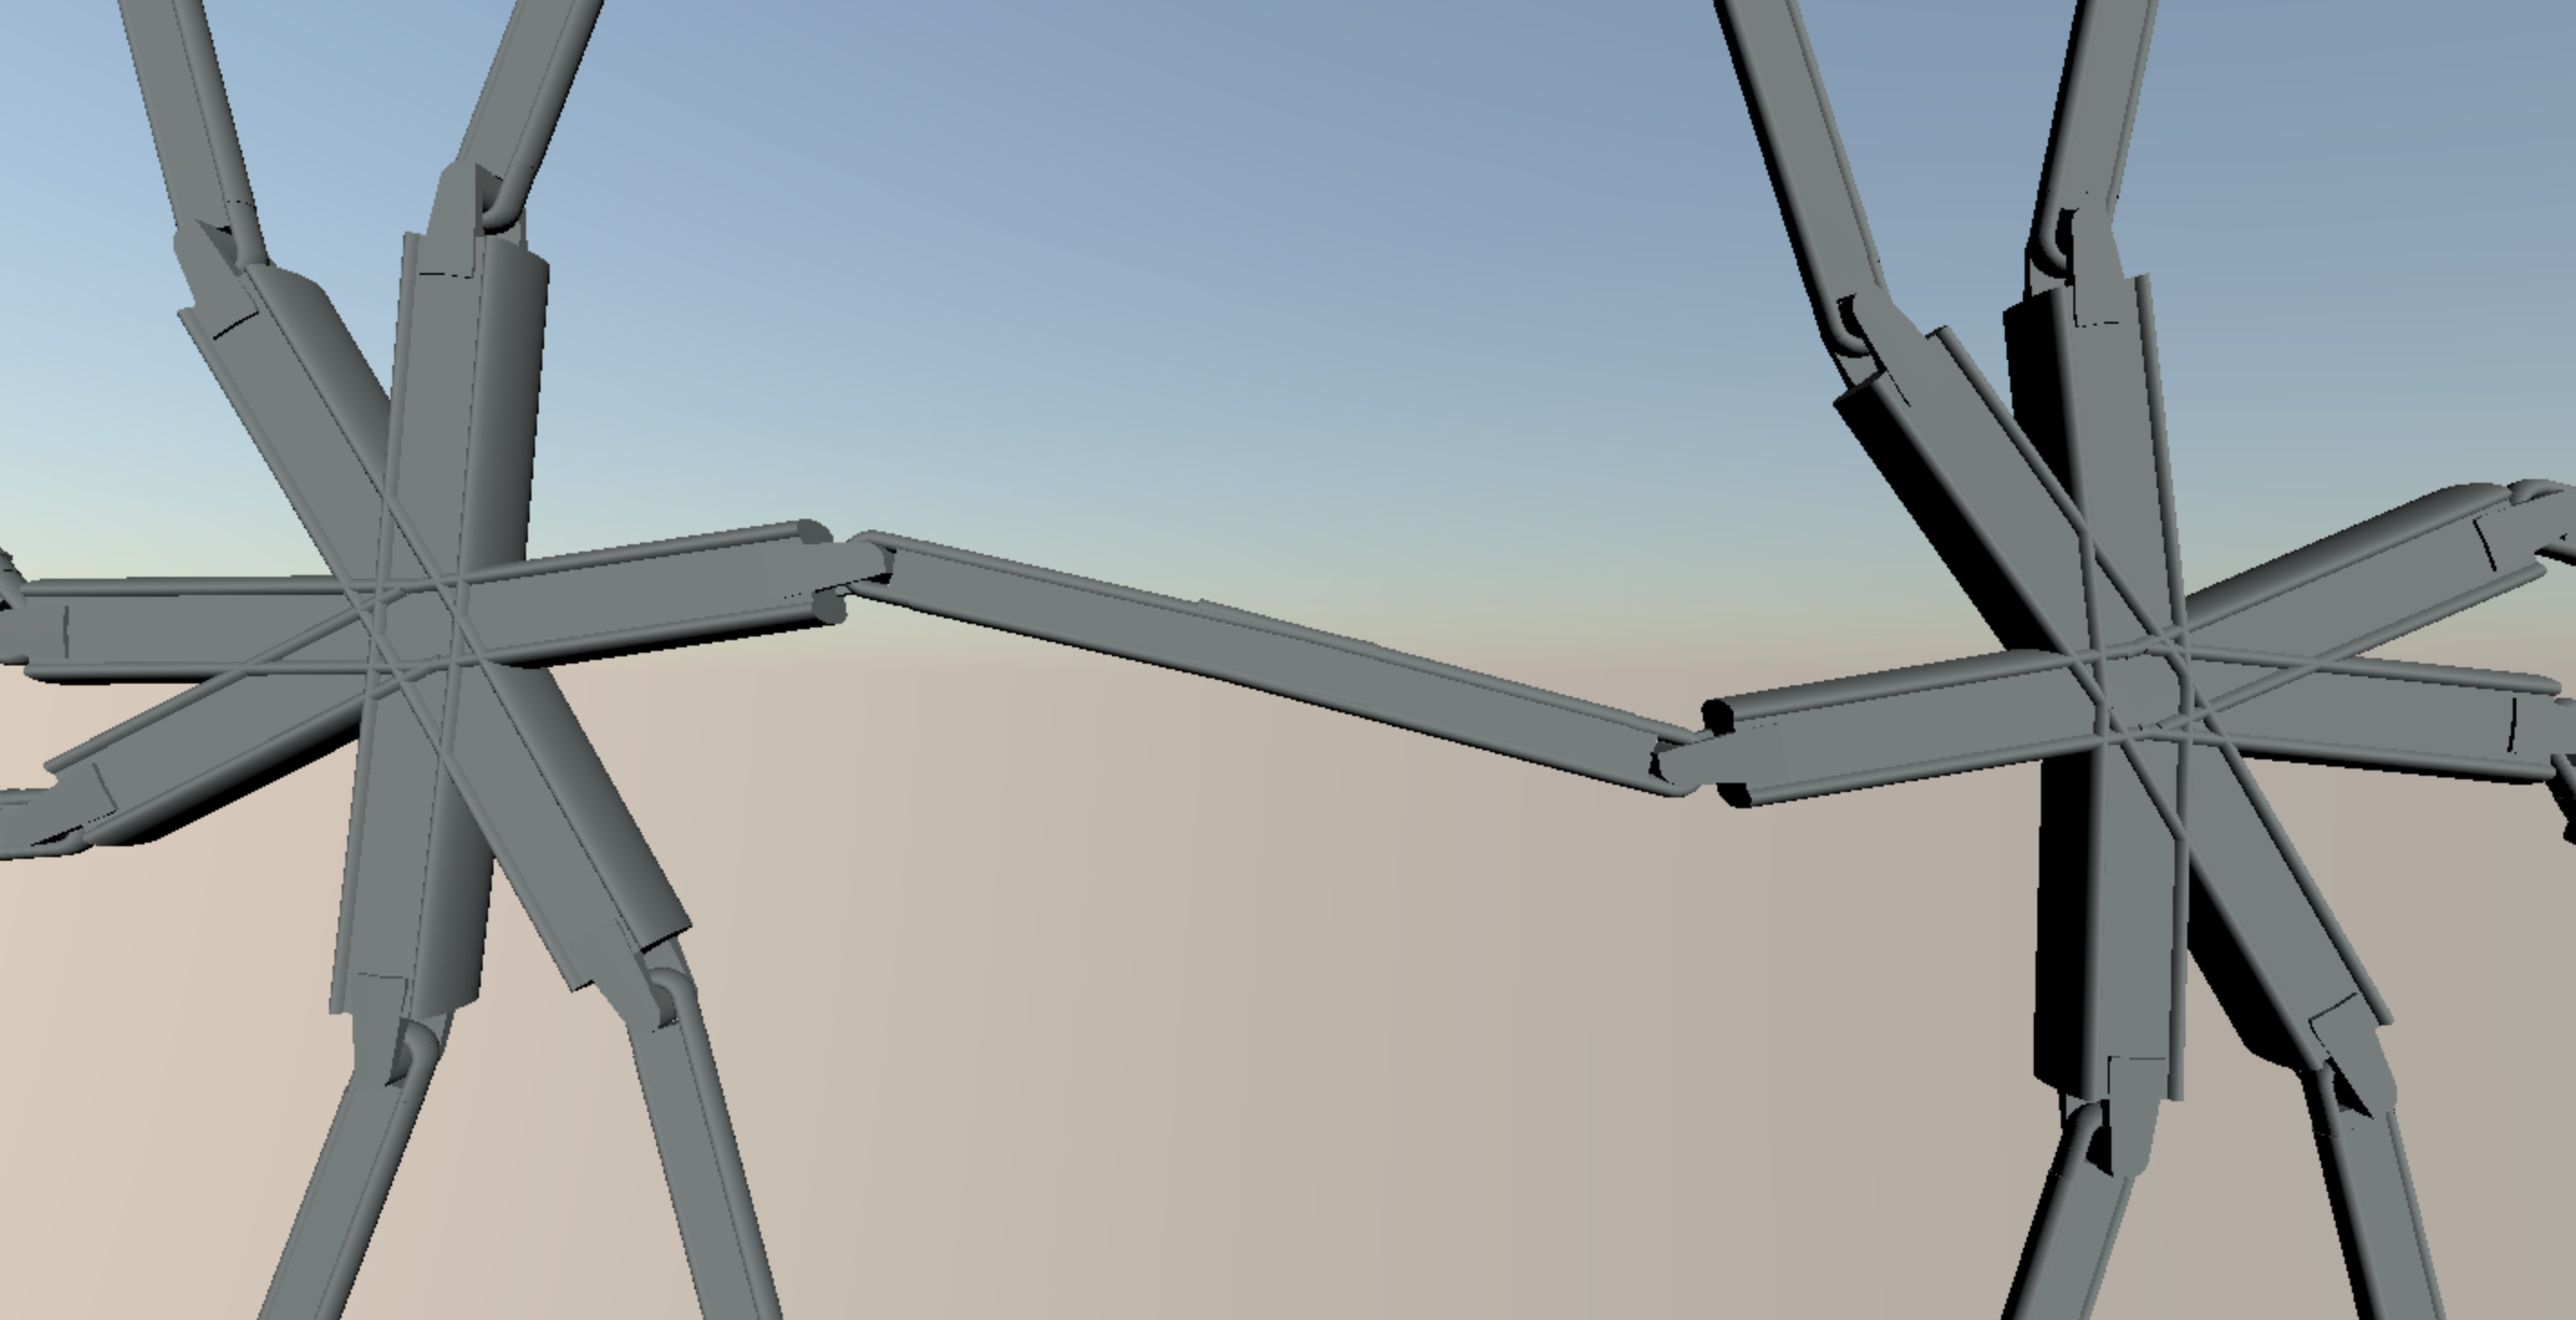
\includegraphics[scale=0.1]{example1.png}

\pagebreak

\printbibliography

\nocite{*}

\end{document}
